\documentclass [a4paper, 10pt]{article}
\usepackage{fullpage}
\usepackage[utf8]{inputenc}
\usepackage{polski}
\usepackage{hyperref}
\usepackage[usenames,dvipsnames]{color}
\hypersetup{
    bookmarks=true,         % show bookmarks bar?
    unicode=false,          % non-Latin characters in Acrobat’s bookmarks
    pdftoolbar=true,        % show Acrobat’s toolbar?
    pdfmenubar=true,        % show Acrobat’s menu?
    pdffitwindow=false,     % window fit to page when opened
    pdfstartview={FitH},    % fits the width of the page to the window
    pdftitle={Zadanie domowe},    % title
    pdfauthor={Stanisław Chmiela},     % author
    pdfsubject={Zadanie domowe},   % subject of the document
    pdfcreator={Stanisław Chmiela},   % creator of the document
    pdfproducer={Stanisław Chmiela}, % producer of the document
    pdfkeywords={matematyka} {zadanie domowe}, % list of keywords
    pdfnewwindow=false,      % links in new window
    colorlinks=true,       % false: boxed links; true: colored links
    linkcolor=BrickRed,          % color of internal links
    citecolor=PineGreen,        % color of links to bibliography
    filecolor=RawSienna,      % color of file links
    urlcolor=MidnightBlue      % color of external links
}
\usepackage[pdftex]{graphicx}
\usepackage{wrapfig}
\usepackage{float}
\usepackage{tikz}
\usepackage{amsfonts}
\usepackage{multicol}
\usetikzlibrary{shapes,snakes,trees}
\usepackage{amsmath}
\linespread{1.3}
\author{Stanisław Chmiela}
\title{Zadanie domowe}
\begin{document}
\maketitle

\tikzstyle{mybox} = [draw=black, fill=white, thick,
    rectangle, rounded corners, inner sep=10pt, inner ysep=10pt]
\tikzstyle{fancytitle} =[fill=black, rounded corners, text=white, font=\bfseries]
\begin{multicols*}{2}

\begin{tikzpicture}
\node [mybox] (box){%
    \begin{minipage}{0.4\textwidth}
    $\Omega = \{\{a,b,c\}: a,b,c \in \{1,3,4,5,6\}, a \neq b \neq c \neq a\}$\\
    $\#\Omega = \frac{5\cdot4\cdot3}{3!} = 10$\\
    $A = \{\{a,b,c\}\in \Omega: a+b>c\}$\\
    Oznaczmy przez $A_i$ liczbę takich zbiorów A, dla których największą liczbą będzie $i$.
    $A_1 = A_3 = A_4 = 0$\\
    $A_5 = 1$, mamy jeden zbiór: $\{3,4,5\}$\\
    $A_6 = 3$, mamy trzy takie zbiory: $\{4,5,6\}, \{3,4,6\}, \{3,5,6\}$\\
    $|A| = |A_1| + |A_3| + |A_4| + |A_5| + |A_6| = 4$\\
    $P(A) = \frac{\#A}{\#\Omega} = \mathbf{\frac4{10}}$
    \end{minipage}
};
\node[fancytitle, right=10pt] at (box.north west) {Zadanie 6.41 a)};
\end{tikzpicture}

\begin{tikzpicture}
\node [mybox] (box){%
    \begin{minipage}{0.4\textwidth}
    $\Omega = \{\{a,b,c\}: a,b,c \in \{1,3,4,5,6\}, a \neq b \neq c \neq a\}$\\
    $\#\Omega = \frac{5\cdot4\cdot3}{3!} = 10$\\
    $A = \{\{a,b,c\}\in \Omega: a^2 + b^2 = c^2\}$\\
    Wśród wszystkich trójek liczb zawierających się w $\{1,3,4,5,6\}$ tylko jedna spełnia równanie $a^2 + b^2 = c^2$. Jest to trójka $\{3,4,5\}$.
    $|A| = 1$\\
    $P(A) = \frac{\#A}{\#\Omega} = \mathbf{\frac1{10}}$
    \end{minipage}
};
\node[fancytitle, right=10pt] at (box.north west) {Zadanie 6.41 b)};
\end{tikzpicture}

\begin{tikzpicture}
\node [mybox] (box){%
    \begin{minipage}{0.4\textwidth}\textit{Pozdro dla Grabcia za wytknięcie błędu, w talii jest 16 figur.}
    Figur w talii jest 16. Asów jest 4. Prawdopodobieństwo wyciągnięcia asa, jeśli wiemy, że karta jest figurą wynosi $P(A) = \mathbf{\frac14}$.
    \end{minipage}
};
\node[fancytitle, right=10pt] at (box.north west) {Zadanie 7.2};
\end{tikzpicture}

\begin{tikzpicture}
\node [mybox] (box){%
    \begin{minipage}{0.4\textwidth}
    Przeanalizujmy to zadanie za pomocą drzewka stochastycznego:
    
\tikzstyle{level 1}=[level distance=2.5cm, sibling distance=2.5cm]
\tikzstyle{level 2}=[level distance=2.5cm, sibling distance=2cm]
\tikzstyle{bag} = [text width=4em, text centered]
\begin{tikzpicture}[grow=down, sloped]
\node[bag] {$\mathbf{3B, 3Z, 3C}$}
    child {
        node[bag] {\textbf{Zielona}\\$\mathbf{3B, 2Z, 3C}$}        
            child {
                node[bag] {\textbf{Zielona}\\$\mathbf{3B, 1Z, 3C}$}
                edge from parent
                node[above] {$\mathbf{\frac{2}{8}}$}
                node[below]  {}
            }
            child {
                node[bag] {Niezielona\\}
                edge from parent
                node[above] {$\frac{6}{8}$}
                node[below]  {}
            }
            edge from parent 
            node[above] {$\mathbf{\frac39}$}
            node[below]  {}
    }
    child {
        node[bag] {Niezielona}        
        edge from parent         
            node[above] {$\frac{6}{9}$}
            node[below]  {}
    };
\end{tikzpicture}
\\
Prawdopodobieństwo, że wylosujemy dwie zielone kule wynosi $P(A) = \frac39\cdot\frac28 = \mathbf{\frac1{12}}$.
    \end{minipage}
};
\node[fancytitle, right=10pt] at (box.north west) {Zadanie 7.5};
\end{tikzpicture}


\begin{tikzpicture}
\node [mybox] (box){%
    \begin{minipage}{0.4\textwidth}
    \textbf{Dane:}\\
    $P(A\cap B) = \frac13, P(A\cup B) = \frac56, P(B') = \frac12$.\\
    \textbf{Szukane:}\\
    $P(A), P(B), P(A|B)$.\\
    \textbf{Rozwiązanie:}\\
    $P(B) = 1-P(B') = 1-\frac12 = \mathbf{\frac12}$\\
    $P(A) = P(A\cup B) - P(B) + P(A\cap B) = \frac56 - \frac12 + \frac13 = \mathbf{\frac23}$\\
    $P(A|B) = \frac{P(A\cap B)}{P(B)} = \frac{\frac13}{\frac12} = \mathbf{\frac23}$
    \end{minipage}
};
\node[fancytitle, right=10pt] at (box.north west) {Zadanie 7.8};
\end{tikzpicture}


\end{multicols*}
\begin{tikzpicture}
\node [mybox] (box){%
    \begin{minipage}{0.9\textwidth}
   \begin{center} \begin{tikzpicture} 
    \pgfmathsetmacro{\cubex}{2}
\pgfmathsetmacro{\cubey}{2}
\pgfmathsetmacro{\cubez}{2}
\draw[black,fill=white, sharp corners] (0,0,0) -- ++(-\cubex,0,0) -- ++(0,-\cubey,0) -- ++(\cubex,0,0) -- cycle;
\draw[black,fill=white, sharp corners] (0,0,0) -- ++(0,0,-\cubez) -- ++(0,-\cubey,0) -- ++(0,0,\cubez) -- cycle;
\draw[black,fill=white, sharp corners] (0,0,0) -- ++(-\cubex,0,0) -- ++(0,0,-\cubez) -- ++(\cubex,0,0) -- cycle;
    \end{tikzpicture} 
    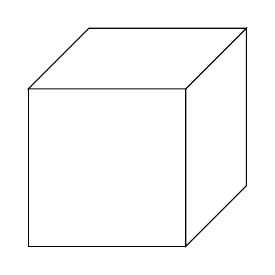
\begin{tikzpicture}
    \pgfmathsetmacro{\cubex}{2}
\pgfmathsetmacro{\cubey}{2}
\pgfmathsetmacro{\cubez}{2}
\draw[black,fill=white, sharp corners] (0,0,0) -- ++(-\cubex,0,0) -- ++(0,-\cubey,0) -- ++(\cubex,0,0) -- cycle;
\draw[black,fill=white, sharp corners] (0,0,0) -- ++(0,0,-\cubez) -- ++(0,-\cubey,0) -- ++(0,0,\cubez) -- cycle;
\draw[black,fill=white, sharp corners] (0,0,0) -- ++(-\cubex,0,0) -- ++(0,0,-\cubez) -- ++(\cubex,0,0) -- cycle;
    \end{tikzpicture}
    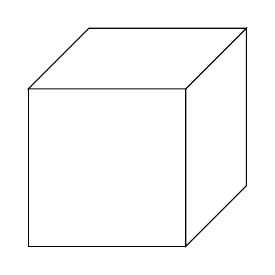
\begin{tikzpicture}
    \pgfmathsetmacro{\cubex}{2}
\pgfmathsetmacro{\cubey}{2}
\pgfmathsetmacro{\cubez}{2}
\draw[black,fill=white, sharp corners] (0,0,0) -- ++(-\cubex,0,0) -- ++(0,-\cubey,0) -- ++(\cubex,0,0) -- cycle;
\draw[black,fill=white, sharp corners] (0,0,0) -- ++(0,0,-\cubez) -- ++(0,-\cubey,0) -- ++(0,0,\cubez) -- cycle;
\draw[black,fill=white, sharp corners] (0,0,0) -- ++(-\cubex,0,0) -- ++(0,0,-\cubez) -- ++(\cubex,0,0) -- cycle;
    \end{tikzpicture}
    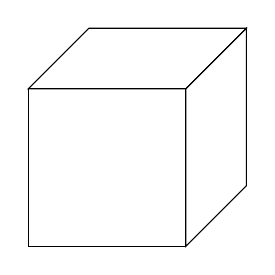
\begin{tikzpicture}
    \pgfmathsetmacro{\cubex}{2}
\pgfmathsetmacro{\cubey}{2}
\pgfmathsetmacro{\cubez}{2}
\draw[black, sharp corners] (0,0,0) -- ++(-\cubex,0,0) -- ++(0,-\cubey,0) -- ++(\cubex,0,0) -- cycle;
\draw[black, sharp corners] (0,0,0) -- ++(0,0,-\cubez) -- ++(0,-\cubey,0) -- ++(0,0,\cubez) -- cycle;
\draw[black, sharp corners] (0,0,0) -- ++(-\cubex,0,0) -- ++(0,0,-\cubez) -- ++(\cubex,0,0) -- cycle;
    \end{tikzpicture}\end{center}
    Są tylko cztery możliwe ustawienia wierzchołków trójkąta – reszta jest ich przesunięciem lub obróceniem.
    \begin{enumerate}
        \item Trójkąt „należy” do wierzchołka, gdy przy wierzchołku jest kąt prosty. Każdy wierzchołek może utworzyć trzy takie trójkąty. $8\cdot3 = 24$ trójkatów.
        \item Trójkąt „należy” do wierzchołka, gdy przy jego ścianie nie ma innych wierzchołków trójkąta. Każdy wierzchołek może tworzyć dwa takie trójkąty. $8\cdot2 = 16$ trójkątów.
        \item Takich trójkątów jest po prostu 8. $8$ trójkątów.
        \item Trójkąt „należy” do wierzchołka, gdy przy jego ścianie nie ma innych wierzchołków trójkąta. Każdy wierzchołek może tworzyć jeden taki trójkąt. $8\cdot 1 = 8$ trójkątów.
    \end{enumerate}
    Wszelkich trójkątów możemy utworzyć $|\Omega| = \frac{8\cdot7\cdot6}{3!} = 8\cdot 7 = 56$.
    \\\textbf{Podpunkt a)} Prostokątnymi trójkątami są tylko trójkąty z punktów 1 oraz 2. Trójkątów takich jest 40. Zatem $P(A) = \frac{40}{56} = \mathbf{\frac57}$.
    \\\textbf{Podpunkt b)} Równoramiennymi trójkątami są trójkąty z punktów 1, 3 i 4. Liczba takich trójkątów: 40. Zatem $P(B) = \mathbf{\frac57}$.
    \end{minipage}
};
\node[fancytitle, right=10pt] at (box.north west) {Zadanie 6.44};
\end{tikzpicture}

\end{document}
